\chapter{week2}

\section{Tuesday}\index{Tuesday_lecture}
\subsection{Quasi-linear Equations}
Review: last week we have learn how to solve the following PDE and get the solution along characteristic curves.
\[\uy+c\ux=0\qquad x\ux+y\uy=u
\]
\begin{figure}[H]
\centering
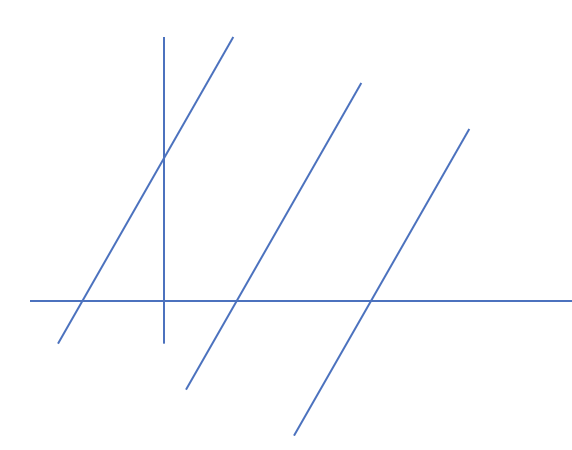
\includegraphics[width=3cm]{week2_tuesday1}
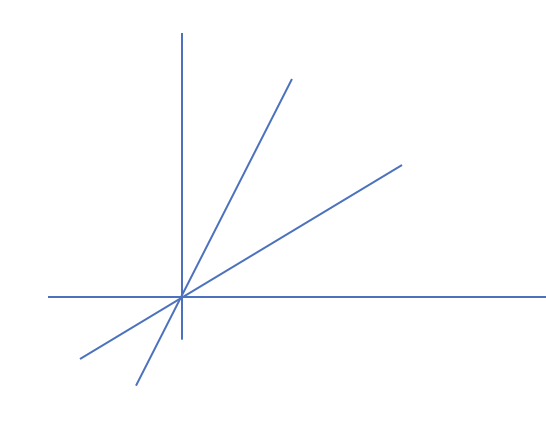
\includegraphics[width=3cm]{week2_tuesday2}
\end{figure}
\[a(x,y,u)\ux+b(x,y,u)\uy=c(x,y,u)
\]
This is what we called quasi-linear equation. At this time, I have to quote our textbook p9 since I cannot explain what professor said better than it does.
\begin{figure}[H]
\centering
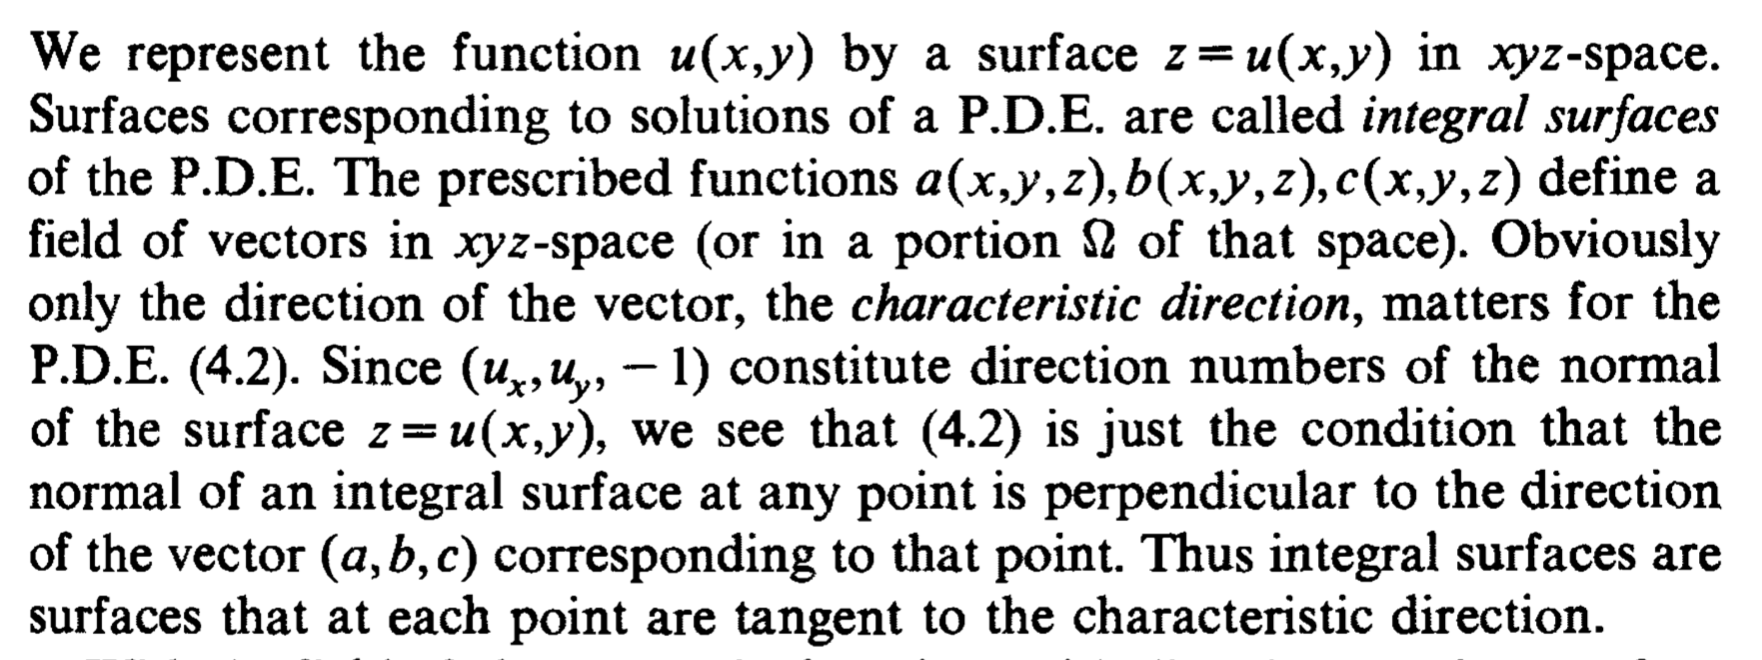
\includegraphics[width=15cm]{week2_tuesday3}
\end{figure}
\begin{figure}[H]
\centering
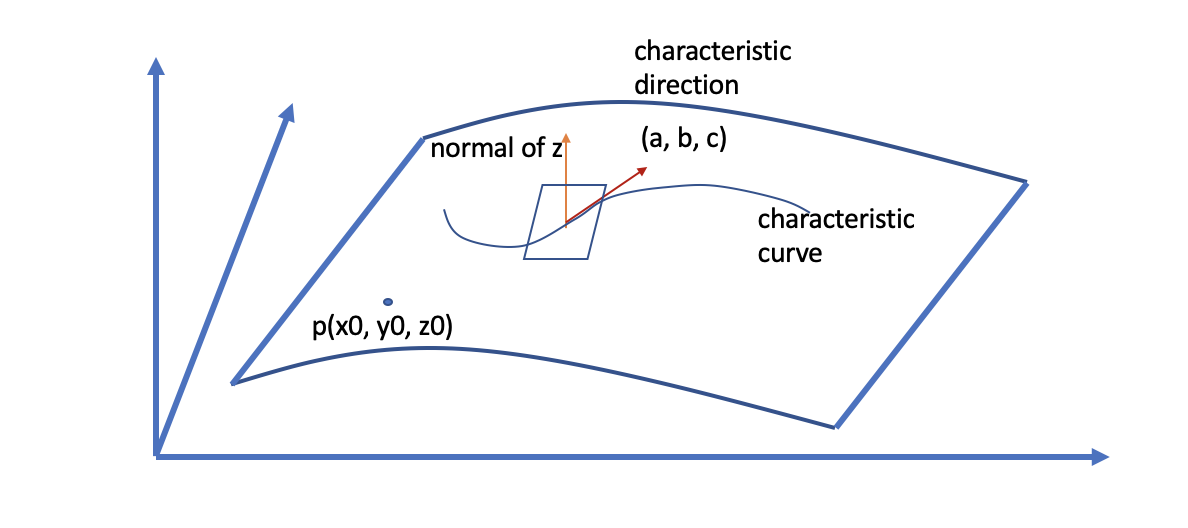
\includegraphics[width=15cm]{week2_tuesday4}
\end{figure}
Next we are going to show that the integral surface, that is the solution $u$ we want, is the union of characteristic curves.
\begin{theorem}
If a characteristic curve $\mathscr{C}$ has one point on a integral surface $z=u(x,y)$ then $\mathscr{C}$ lies entirely on the surface.

\end{theorem}
\begin{proof}
\[z_0=u(x_0,y_0)
\]
\[\left\{\begin{gathered}\deriv{x}{t}=a(x(t),y(t),u(x_0,y_0))\\\deriv{y}{t}=b(x(t),y(t),u(x_0,y_0))\\x(0)=x_0\\y(0)=y_0\end{gathered}\right.
\]
This is a system of odes, there is a solution ($x(t),y(t)$) when $t$ is around 0.\\
This gives us a curve $(x(t),y(t),u(x(t),y(t)))$ lies on the integral surface.\\
Claim: It's a characteristic curve.
\[z(t)=u(x(t),y(t))
\]
\[\deriv{z}{t}=\ux\deriv{x}{t}+\uy\deriv{y}{t}=a\ux+b\uy=c
\]



\end{proof}
\subsection{Cauchy Problem}
``Finding the function $u(x,y)$ for given data $f(s)$, $g(s)$, $h(s)$ constitutes the \text{\it Cauchy problem} for quasi-linear equation.'' (John, 1982, p.9)\\ The following $\varphi, \psi, \rho$ are $f, g, h$ correspondingly.\\
To solve the Cauchy problem, it suffices to require that $(\psi\p,\varphi\p)\&(a,b)$ are linearly independent.\\The
\[\left\{\begin{gathered}\deriv{\bar{X}}{t}=a(\bar{X},\bar{Y},Z)\\\deriv{\bar{Y}}{t}=b(\bar{X},\bar{Y},Z)\\\deriv{\bar{z}}{t}=c(\bar{X},\bar{Y},Z)\\\bar{X}(s,0)=\varphi(s)\\\bar{Y}(s,0)=\psi(s)\\\bar{Z}(s,0)=\rho(s)\end{gathered}\right.
\]
Existence and uniqueness theorem for ODE.\\
$\Rightarrow$ For every $s$, $\exists$ one solution $(\bar{X}(s,t),\bar{Y}(s,t),z(s,t))$. In order to make $u(x,y)=z(s(x,y),t(x,y))$ is the case. We need implicit function theorem which makes us able to write $s, t$ as a function of $(x,y)$
\[\begin{vmatrix}\frac{\partial{\bar{X}}}{\partial{s}}&\frac{\partial{\bar{X}}}{\partial{t}}\\\frac{\partial{\bar{Y}}}{\partial{s}}&\frac{\partial{\bar{Y}}}{\partial{t}}\end{vmatrix}=\begin{vmatrix}\varphi\p&a\\\psi\p&b\end{vmatrix}\neq0
\]
\begin{example}
\[\uy+u\ux=0, \quad u(x,0)=f(x)\]
\[\deriv{x}{t}=z,~\deriv{y}{t}=1,~\deriv{z}{t}=0
\]
$z$ is constant in $t$. $z(s, 0)=f(s)\Rightarrow z(s,t)=f(s)$.
\[\dakuohao{x(s,0)=s~\Rightarrow~x(s,t)=f(s)t+s}{y(s,0)=0~\Rightarrow~y(s,t)=t}\rightarrow ~s=x-f(s)t=x-f(s)y=x-zy
\]
\[z(s,0)=f(s)\Rightarrow z(s,t)=f(s)=f(x-zy)
\]
\[u(x,y)=f(x-uy)
\]
Characteristic curve
\[f(s_2)>f(s_3)
\]
\[\frac{1}{f(s_2)}<\frac{1}{s_3}
\]
Why it is called a ``Shock''?\\The reason is that: for same $(x,y)$ $z$ should be the same. However, from the graph we can see there are two $z$ corresponds to the same point marked by the circle. Therefore, the solution does't exist.
\begin{figure}[H]
\centering
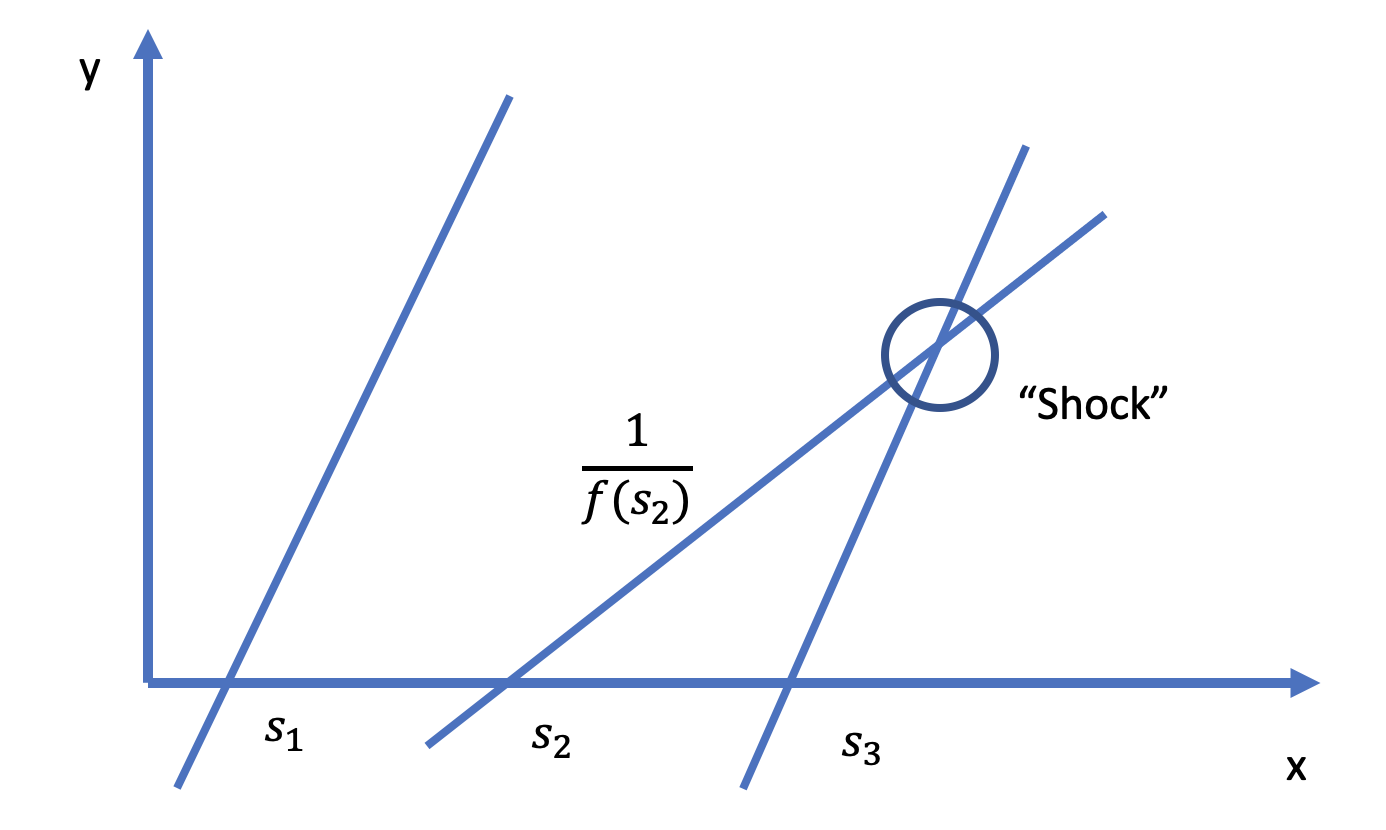
\includegraphics[width=8cm]{week2_tuesday5}
\end{figure}



\end{example}
